\section{\MakeUppercase{Implementation Details}}
\subsection{Dataset Generator Implementation}
Initially, we collected the multiple number of hand-drawn sketches for the each element under consideration. Our focus was on selecting elements that provided the most efficient and informative structural layout for the user Interface. Once we finalized the core set of elements, the individual sketches are combined to create a many numbers of sketch wireframe required to train our Transformer model.  This approach allows us to create a larger and diverse dataset that contains different design possibilities and layout variations.
\subsubsection{Steps taken in Dataset Generation}
\textbf{Random DSL generator}\\
The first step in the data generation process is the creation of the Domain-Specific Language (DSL) code. This DSL code was generated using a set of custom-made rules designed to ensure effective representation of web page layouts. The rules were created to allow different combinations of elements, ensuring a variety of layout that represents the User Interface. Each generated DSL code was unique, with varying arrangements of UI components so that it provides the broad spectrum of design possibilities. The DSL generation process involves refinement and testing to be sure that the generated code was both meaningful and represents the real-world web layouts.

\textbf{Compiling the DSL Code}\\
Once the DSL code was generated, the next step is to compile or map it to the corresponding HTML code. This process involved translating the high-level DSL representation into a concrete and functional HTML structure which can be used by the browers to give User Interface. During the compilation phase, special attention was given to maintaining semantic correctness and ensuring that the generated HTML structure follows rules of design of web page and aligned with best practices in web development. The compiled HTML code served as the foundation upon which additional styling and interactivity were layered.

\textbf{Rendering the produced HTML Code}\\
After compiling the DSL code into HTML, the resulting web pages were rendered in a Chrome browser. During the rendering process, a specialized CSS file was applied to style the elements, ensuring a visually distinct and well-structured layout is obtained. Different elements within the page were rendered with specific background colors with the help of specialized CSS, which played a crucial role in subsequent processing steps. Additionally, a JavaScript file was used to dynamically assign random height, width, and positioning values to each element, introducing variability and making the dataset more comprehensive. Once the elements were properly rendered and positioned, screenshots of the pages were captured for further processing.

\textbf{Finding the outline of the different element}\\
To identify and extract the individual elements from the rendered pages, a contour detection technique is used. This involved filtering out the background colors assigned during the rendering phase and using image processing techniques to detect the contours of each UI component. Through this approach, the precise dimensions and positions of various elements were obtained. These bounding boxes provides critical information which is later used to align the hand-drawn sketches with the corresponding UI components.

\textbf{Placement of hand-drawn sketch}\\
Once the bounding boxes for each element are identified, the next step is to overlay the hand-drawn sketches onto the detected elements. To achieve this, the aspect ratios of the hand-drawn sketches are compared with those of the bounding boxes. The sketches are then sorted based on the closest matching aspect ratios to ensure an optimal fit. From the top-ranked sketches, a random selection of up to eight sketches is made, and one of them is placed within the corresponding bounding box. This step ensures a realistic and visually appealing integration of the sketches within the generated layouts.

\textbf{Rules for creating DSL}\\
To ensure consistency and structure in the generated web layouts, a set of rules and guidelines is established for DSL generation. The structure was based on a hierarchical representation of webpage elements, where each key element had a predefined set of possible child elements. For example, the 'root' element could contain 'header', 'container', and 'footer' sections, while a 'row' could include various sizes of 'div' elements. The layout generation also incorporated a 12-column grid system, which is widely used in responsive web design. This grid-based approach allowed for flexible and adaptive layouts while maintaining a sense of order and balance.
Furthermore, constraints are introduced to govern the occurrence and arrangement of elements. These constraints defined the minimum and maximum number of occurrences for each component, the order in which child elements should appear, and the allowable combinations for dividing rows into columns. By enforcing these rules, we ensured that the generated layouts were both diverse and logically structured. The flexibility provided by these constraints allowed for a wide range of layout variations while maintaining essential structural integrity.
Overall, the structured approach for dataset generation enable us to create a rich and diverse set of training data that captured a wide variety of design possibilities. This process laid the groundwork for training our Transformer model effectively, ensuring it could generalize well across different UI layouts and design elements.
\subsection{Model Implementation}
We have developed a transformer-based architecture designed to convert sketch images into DSL code. The architecture consists of an encoder that processes the input images (sketches) and a decoder which is responsible for generating the corresponding DSL code. To achieve high accuracy and efficiency, our model leverages Convolutional Neural Networks (CNNs) for feature extraction from images and transformer layers for sequence modeling. This combination allows the model to effectively translate visual representations into structured textual output, which is the DSL code.
\subsubsection{Input Processing}
The model is designed to accept two types of inputs for the training of the model. This is the processing that is done in the training phase. Otherwise, we just have to input the image:
\begin{enumerate}
    \item \textbf{Image Input}
    The first input to the model is a grayscale sketch image with dimensions (None, 850, 600, 1). Each sketch serves as a visual representation of a UI layout and is processed through the CNN layers to extract meaningful spatial features and patterns.
    \item \textbf{Text Input}
    The second input is the textual representation of the DSL code associated with the given sketch. It has a shape of (None, 120), where each sequence represents the structural layout and element relationships defined in the DSL format. This input acts as a ground truth reference during the training process.The input processing pipeline involves several key steps, including image normalization, tokenization of the DSL text input to enable efficient processing by the transformer layers. By integrating both image and text inputs, the model is trained to establish a strong correlation between visual layouts and their corresponding code representations, which provides the accurate and reliable predictions.
\end{enumerate}
\subsubsection{Convolutional Tokenizer}
The Convolutional Tokenizer is the first critical component of our transformer-based architecture, which is responsible for processing the input sketch images and transforming them into meaningful feature representations. It helps in focusing on the feature that are important for the DSL generations so, we do not require large number of input images to train the transformer model. This custom layer contains a series of convolutional and pooling operations to convert the 2D grayscale image into a sequence of feature vectors. The output of the tokenizer has a shape of (None, 513, 128), which indicates that the input image is transformed into 513 tokens, each represented by a feature vector of 128 dimensions. This transformation is crucial as it prepares the data for further processing by the subsequent transformer layers. This layers encode the features present in the image into a feature vectors.

\textbf{Convolutional Layers}\\
The Convolutional Tokenizer comprises multiple convolutional layers (Conv2D), each of which are designed to extract hierarchical features from the input image. The number of filters increases as the network goes deeper, which helps in richer and more abstract representation of the image features. Each convolutional layer is followed by zero-padding and max-pooling operations, which help in preserving spatial dimensions and capturing essential patterns while also reducing computational complexity. Dropout layers are also placed within the network to mitigate the risk of overfitting and improve generalization.

\textbf{Layer-wise Breakdown}
\begin{enumerate}[label=\textbf{\roman*})]
    \item \textbf{First Convolutional Layer:}
    \begin{itemize}
        \item Filters: 32
        \item Kernel Size: 7x7
        \item Stride: 1
        \item Padding: None initially, followed by ZeroPadding2D of 1 to preserve spatial dimensions.
        \item Activation Function: ReLU
        \item Pooling: MaxPooling2D with a window size of 3x3 and a stride of 2.
    \end{itemize}
    In this initial layer, the large kernel size of 7x7 is used, which allows the model to capture broader structural features from the sketch image. The addition of zero-padding ensures that the spatial dimensions remain intact, while max-pooling helps in reducing the feature map size and computational load.

    \item \textbf{Second Convolutional Layer:}
    \begin{itemize}
        \item Filters: 64
        \item Kernel Size: 5x5
        \item Stride: 1
        \item Padding: None initially, followed by ZeroPadding2D of 1.
        \item Activation Function: ReLU
        \item Pooling: MaxPooling2D with a 3x3 pooling window and stride of 2.
        \item Dropout: Applied with a rate of 0.1.
    \end{itemize}
    The second layer increases the depth of feature maps, allowing the model to learn more complex patterns. Dropout is applied after this layer to prevent overfitting by randomly deactivating some neurons during training, encouraging the network to learn more robust features.

    \item \textbf{Third Convolutional Layer:}
    \begin{itemize}
        \item Filters: 64
        \item Kernel Size: 3x3
        \item Stride: 1
        \item Padding: None initially, followed by ZeroPadding2D of 1.
        \item Activation Function: ReLU
        \item Pooling: MaxPooling2D with a 3x3 pooling window and stride of 2.
    \end{itemize}
    With a smaller kernel size of 3x3, the third layer focuses on detecting finer details in the image while maintaining an efficient processing pipeline through down-sampling via max-pooling.

    \item \textbf{Fourth Convolutional Layer:}
    \begin{itemize}
        \item Filters: 128
        \item Kernel Size: 3x3
        \item Stride: 1
        \item Padding: None initially, followed by ZeroPadding2D of 1.
        \item Activation Function: ReLU
        \item Pooling: MaxPooling2D with a 3x3 pooling window and stride of 2.
        \item Dropout: Applied with a rate of 0.1.
    \end{itemize}
    The fourth layer further enhances the feature representation by increasing the number of filters to 128. This allows the model to detect complex patterns, edges, and finer textures. The dropout layer once again aids in generalization.

    \item \textbf{Fifth Convolutional Layer:}
    \begin{itemize}
        \item Filters: 128
        \item Kernel Size: 3x3
        \item Stride: 1
        \item Padding: None initially, followed by ZeroPadding2D of 1.
        \item Activation Function: ReLU
        \item Pooling: MaxPooling2D with a 3x3 pooling window and stride of 2.
    \end{itemize}
\end{enumerate}
    The final convolutional layer retains the same number of filters as the previous layer, ensuring consistency in feature extraction and maintaining high-dimensional feature representations. The resulting feature maps undergo max-pooling to down-sample and prepare them for the subsequent flattening process.

\textbf{Flattening the Output}\\
After passing through all convolutional and pooling layers, the output feature maps are flattened into a shape of (513, 128). This transformation converts the spatially distributed feature maps into a sequence of 513 tokens, each represented by a 128-dimensional feature vector. This sequential representation is then fed into the transformer model for further processing and translation into DSL code.
The Convolutional Tokenizer plays a crucial role in bridging the gap between raw image input and the transformer-based sequence processing model. Its structured design ensures efficient feature extraction, dimensionality reduction, and effective preparation of input data for downstream tasks. By incorporating a combination of convolutional layers, pooling operations, and dropout mechanisms, our tokenizer ensures high performance, robustness, and scalability for processing sketch images of varying complexity and style.

\subsubsection{Positional Embedding}
After the convolutional tokenization process, positional encoding is applied to the token embeddings to incorporate spatial information. Since transformers do not inherently capture the order or spatial relationships of input sequences, the use of positional encoding is essential for enabling the model to understand the positional relationships between different parts of the image.\\
We have used sinusoidal positional encoding, which is a widely used technique that provides a unique representation for each position in the input sequence. The sinusoidal encoding functions are designed to produce continuous and periodic values, which allow the model to generalize to sequences of varying lengths and effectively capture patterns in spatial arrangements.

\textbf{Sinusoidal Positional Encoding}\\
This encoding scheme allows each position to have a unique representation based on sine and cosine functions of different frequencies, enabling the model to distinguish between different token positions efficiently.

\textbf{Combining Tokenized Features with Positional Encoding}\\
Once the token embeddings are obtained from the convolutional tokenizer, the positional encodings are added element-wise to the feature vectors. This addition allows the model to retain positional context alongside the extracted features, enhancing its capability to understand spatial dependencies in the sketch images.
The integration of positional embeddings is crucial in ensuring that the model effectively captures both local and global structures within the image layout, which is fundamental for accurate DSL code generation. The combined representation is then passed to the transformer encoder for further processing, where self-attention mechanisms utilize both feature and positional information to derive meaningful relationships among different elements.


\subsubsection{Encoder}
The encoder in our model consists of three transformer blocks, each of which are designed to process the tokenized image data efficiently. Every block in the encoder follows a structured approach that includes several critical components: layer normalization, multi-head attention (self-attention), residual connections, and a \gls{ffnn}.
The encoder is responsible for transforming the input image tokens of shape (513x128) into a meaningful representation that the decoder can further utilize for DSL code generation. The output of each encoder block maintains the same shape of (513x128), preserving spatial consistency while enriching feature representation.

\textbf{Components of the Transformer Encoder}
\begin{enumerate}[label=\textbf{\roman*})]
    \item \textbf{Layer Normalization}
    \begin{itemize}
        \item Each layer normalization operation consists of 256 trainable parameters and serves to normalize inputs across the 128 feature dimensions.
        \item This normalization step is crucial for improving training stability by reducing internal covariate shifts, allowing the model to converge faster and more efficiently.
    \end{itemize}
    
    \item \textbf{Multi-head Attention (Self-attention)}
    \begin{itemize}
        \item The multi-head attention mechanism is a key component in capturing dependencies across different token positions within the sequence.
        \item Each multi-head attention layer has 329,728 parameters, contributing significantly to the model's ability to learn complex relationships.
        \item We have employed 5 attention heads, which allows the model to focus on multiple aspects of the input simultaneously.
        \item The input and output dimensions for the attention layer remain consistent at (513x128), ensuring no loss of spatial or feature-based information.
    \end{itemize}
    
    \item \textbf{Residual Connections}
    \begin{itemize}
        \item To facilitate gradient flow and prevent vanishing gradients, residual connections are used.
        \item These connections add the input of the attention layer (513x128) directly to its output, effectively bypassing the complex transformations and ensuring that important lower-level features are preserved throughout the layers.
    \end{itemize}
    
    \item \textbf{Feed-forward Neural Network (FFNN)}\\
    The feed-forward network within each transformer block is composed of two dense layers:
    \begin{enumerate}
        \item \textbf{First Dense Layer:}
        \begin{itemize}
            \item Has a shape of (513x128) and consists of 16,512 parameters.
            \item This layer applies linear transformations to enrich the feature representation.
        \end{itemize}
        
        \item \textbf{Dropout Layer:}
        \begin{itemize}
            \item A dropout layer is applied after the first dense layer to prevent overfitting and improve generalization during training.
        \end{itemize}
        
        \item \textbf{Second Dense Layer:}
        \begin{itemize}
            \item Another dense layer of the same shape (513x128) with 16,512 parameters is applied.
            \item This is followed by another dropout layer to further regularize the model.
        \end{itemize}
    \end{enumerate}
\end{enumerate}Each of the three transformer encoder blocks follows the above structure, progressively refining the image token embeddings while maintaining the original spatial dimensions. This multi-layered processing enables the model to capture both local and global dependencies within the sketch image representations, which is critical for accurate DSL code generation.



\subsubsection{Decoder}

The decoder is more complex. It is designed to generate DSL code sequences from the encoded image representations. It consists of four transformer blocks, each contributing to the sequential processing of the input embedding while attending to the encoder's output. The decoder processes an input sequence of shape (120x128) and interacts with the encoder output of shape (513x128) to produce the final output sequence.
Each block in the decoder includes:
\begin{enumerate}[label=\textbf{\roman*}]
    \item \textbf{Self-attention Layer} \\
    The self-attention mechanism in the decoder is crucial for processing the input sequence by allowing each position to attend to all previous positions. This mechanism ensures that predictions are made based only on preceding tokens, preventing information leakage from future tokens.
    
    \begin{itemize}
        \item The self-attention layer consists of 329,728 parameters, making it a key computational component.
        \item The input and output dimensions of this layer are (120x128).
        \item A masking mechanism is applied to ensure autoregressive decoding, allowing the model to focus solely on past and current tokens.
    \end{itemize}
    
    \item \textbf{Cross-attention Layer} \\
    The cross-attention layer enables the decoder to focus on relevant parts of the encoder's output while generating the target sequence. This layer establishes dependencies between the input image tokens and the generated code sequence.
    
    \begin{itemize}
        \item It contains 329,728 parameters, similar to the self-attention layer.
        \item The layer takes the encoder's output of shape (513x128) as input and processes it alongside the decoder's sequence of shape (120x128).
        \item This mechanism allows the decoder to align each generated token with specific image features.
    \end{itemize}
    
    \item \textbf{Feed-forward Neural Network (FFNN)} \\
    The feed-forward network is used to further refine the features extracted by the attention layers. It consists of two dense layers, each followed by a dropout layer to prevent overfitting and enhance generalization.
    
    \begin{itemize}
        \item Each dense layer has a size of (120x128) and consists of 16,512 parameters.
        \item The first dense layer applies linear transformations, followed by a dropout layer to introduce regularization.
        \item The second dense layer, also followed by dropout, further refines the output before passing it to the next decoder block.
    \end{itemize}
    
    \item \textbf{Layer Normalization and Residual Connections} \\
    Layer normalization ensures stable training by normalizing activations across the feature dimensions, which helps in maintaining consistent gradient flow.
    
    \begin{itemize}
        \item Each layer normalization contains 256 parameters, applied across the 128 feature dimensions.
        \item Residual connections play a crucial role by adding the input of shape (120x128) to the output of each sublayer, preserving important information and improving gradient flow.
    \end{itemize}
\end{enumerate}
Each of the four decoder transformer blocks processes the input embeddings while interacting with the encoder output, gradually refining the generated sequence. With self-attention, cross-attention, feed-forward networks, layer normalization, and residual connections, the decoder is well-equipped to produce accurate DSL code based on the provided sketch image representation.

\subsubsection{Attention Mechanism}
The attention mechanism is a crucial component of our model, facilitating the processing of both input image tokens and the generated DSL code sequences. The model employs several multi-head attention layers, each designed to capture dependencies across the tokenized representations effectively.

\begin{enumerate}[label=\textbf{\roman*})]
    \item \textbf{Attention in the Encoder}\\
    In the encoder, the attention mechanism consists of self-attention layers, which enable each token within the image representation to attend to all other tokens. This allows the model to capture intricate relationships between different parts of the sketch, ensuring a rich feature representation.
    \begin{itemize}
        \item Self-Attention:
        Each token in the sequence of shape (513x128) can interact with every other token, leading to a comprehensive understanding of the entire image layout.
        \item Multi-Head Attention
        Multiple attention heads allow the model to focus on different aspects of the image simultaneously, improving its ability to discern patterns and spatial relationships.
    \end{itemize}
    
    \item \textbf{Attention in the Decoder}\\
    The decoder contains two types of attention mechanisms: self-attention and cross-attention, which work together to generate the target sequence effectively.
    \begin{itemize}
        \item Self-Attention in Decoder:
        The decoder's self-attention layers process the sequence of shape (120x128), enabling each token to attend to previous tokens. This ensures that each predicted token is generated based only on previously seen information, maintaining the autoregressive nature of the sequence generation.
        \item Cross-Attention
        The cross-attention layers allow the decoder to focus on relevant parts of the encoder's output while processing the generated sequence.This mechanism aligns the input sketch features (of shape 513x128) with the generated sequence, ensuring meaningful code generation.
    \end{itemize}
    
    \item \textbf{Multi-Head Attention}
    Each attention layer employs a multi-head mechanism to improve learning by attending to different aspects of the sequence in parallel.
    \begin{itemize}
        \item The number of attention heads used in our model is 5, which enhances the model’s capability to capture diverse relationships.
        \item Each multi-head attention layer in the encoder and decoder contains 329,728 parameters, contributing significantly to the model's complexity and learning power.
        \item The attention layers have consistent input and output dimensions, preserving spatial integrity.
    \end{itemize}
    \end{enumerate}

\subsubsection{Masking}
Masking is a crucial technique which is used in the decoder's self-attention layers to ensure proper sequential processing during the generation of the output sequence. The model implements causal masking, which plays an essential role in autoregressive generation by preventing tokens from accessing future information.

\textbf{Causal Masking in Self-Attention}\\
Causal masking ensures that each position in the output sequence can only attend to previous positions. This is achieved by applying a mask over the attention weights, effectively setting the attention scores of future positions to negative infinity. It prevents information flow from future tokens.

\begin{itemize}
    \item \textbf{Purpose:} It maintains the sequential nature of generation, ensuring that the model predicts each token based solely on previously generated tokens.
    \item \textbf{Implementation:} During the self-attention computation, an upper triangular matrix filled with negative infinity values is added to the attention scores, effectively masking out future positions.
    \item \textbf{Impact:} It helps the model avoid data leakage and ensures that predictions are conditioned correctly, improving the accuracy and coherence of generated sequences.
\end{itemize}

\textbf{Types of Masking Used}

\begin{itemize}
    \item \textbf{Causal Masking:} Applied in the decoder's self-attention to maintain autoregressive properties.
    \item \textbf{Padding Masking:} Optionally used to ignore padding tokens in sequences, ensuring that padding elements do not contribute to the attention mechanism.
\end{itemize}

\textbf{Advantages of Masking}

\begin{itemize}
    \item \textbf{Prevents Information Leakage:} Ensures the model adheres to the sequential generation requirement.
    \item \textbf{Improves Training Stability:} Helps the model learn dependencies in the correct order.
\end{itemize}

By using causal masking in the model, the model can generate the target sequence in an orderly fashion, where each token is predicted based only on past information. This mechanism is crucial for achieving high-quality autoregressive sequence generation in the context of sketch-to-code translation.



\subsubsection{Output Layer}
The final stage of our model is the output layer, which is responsible for generating the predicted DSL code tokens based on the processed input features. This layer plays a critical role in transforming the decoder's learned representations into meaningful output sequences.


\textbf{Structure of the Output Layer:}
\begin{itemize}
    \item The output layer consists of a dense (fully connected) layer with 31 units, which corresponds to the vocabulary size of the output tokens.
    \item The vocabulary size is determined by the number of possible tokens used in the DSL code, minus one to account for the special start token used during sequence generation.
    \item Each unit in the dense layer represents a potential token, and the layer outputs raw logits indicating the likelihood of each token at every position in the output sequence.
\end{itemize}
\textbf{Functionlaity}
\begin{enumerate}[label=\textbf{\roman*})]
    \item \textbf{Logits Generation} 
    \begin{itemize}
        \item The dense layer produces logits for each token position in the sequence, representing the unnormalized probabilities of each token in the vocabulary.
        \item These logits are then processed by a softmax function to convert them into probability distributions over the vocabulary.
    \end{itemize}
    
    \item \textbf{Token Prediction} 
    \begin{itemize}
        \item The highest probability token is selected at each position to construct the final sequence.
        \item This sequence is then used to generate the DSL code corresponding to the input sketch.
    \end{itemize}
\end{enumerate}
\textbf{Training Considerations}
\begin{itemize}
    \item During training, the model uses teacher forcing, where the correct tokens are provided at each step to guide learning.
    \item Cross-entropy loss is used to optimize the output layer by comparing predicted tokens with ground truth tokens.
    \item Dropout techniques and regularization strategies are applied to prevent overfitting and ensure robust generalization.
\end{itemize}
The output layer is a crucial component that bridges the decoder's learned representations and the final code output. By producing logits for each token in the vocabulary, the model can effectively generate accurate DSL code representations based on the provided sketch inputs.
\subsection{Model Complexity}
The designed transformer-based model consists of a total of 3,488,447 trainable parameters, striking a balance between model capacity and computational efficiency. This parameter count reflects the intricacies of the architecture, ensuring that the model can effectively capture the complexity of the sketch-to-code translation task while remaining feasible for training and deployment.

\textbf{Breakdown of Model Complexity}

\begin{enumerate}
    \item \textbf{Encoder Complexity:}
        \begin{itemize}
            \item The encoder comprises multiple convolutional and transformer layers, contributing a significant portion of the total parameter count.
            \item Each convolutional layer extracts hierarchical spatial features from the input sketches, while transformer layers provide contextualized representations. 
        \end{itemize}
    \item \textbf{Decoder Complexity:}
        \begin{itemize}
            \item The decoder consists of several transformer blocks, which include self-attention and cross-attention mechanisms.
            \item These layers allow the decoder to generate coherent DSL code sequences by attending to both past outputs and encoder outputs.
        \end{itemize}
    \item \textbf{Attention Mechanisms:}
        \begin{itemize}
            \item Multi-head attention layers play a crucial role in both encoder and decoder by enabling the model to focus on different aspects of the input.
            \item With five attention heads, the model can efficiently capture relationships between tokens.
        \end{itemize}
    \item \textbf{Feed-forward Networks:}
        \begin{itemize}
            \item Fully connected layers within both the encoder and decoder add to the parameter count, enhancing the representational power of the model.
            \item These layers contribute to non-linear transformations crucial for feature abstraction.
        \end{itemize}
\end{enumerate}

\textbf{Optimization Considerations}
\begin{itemize}
    \item Despite the substantial number of trainable parameters, the model is designed to optimize memory usage and computational efficiency.
    \item Techniques such as dropout and weight regularization are employed to prevent overfitting while maintaining generalization capabilities.
\end{itemize}

The model achieves an optimal balance between complexity and efficiency, ensuring it can process intricate sketch inputs and generate high-quality DSL code within reasonable computational constraints. With 3,488,447 trainable parameters, it is well-suited for the demands of real-world applications.


\subsection{Vocabulary of Model}
The DSL (Domain-Specific Language) used in this project consists of a total of 32 different symbols and words, which serve as the fundamental building blocks for generating structured code from sketch inputs. These elements include both functional commands and structural identifiers essential for the DSL code representation.

\textbf{Special Symbols}\\
The vocabulary includes three special symbols that play critical roles in sequence processing:
\begin{itemize}
    \item \textbf{$<$Start$>$ Symbol:}Assigned the value 31, this token marks the beginning of a sequence and helps the model recognize the start of generation.
    \item \textbf{$<$End$>$ Symbol:}Signals the end of a sequence, indicating when the model should stop generating output.
    \item \textbf{$<$Pad$>$ Symbol:}Assigned the value 0, this token is used to pad shorter sequences to ensure uniform input dimensions, enabling efficient batch processing.
\end{itemize}
\textbf{Textual Representation and Vector Conversion}\\
To process the DSL code efficiently, the textual representation is converted into a numerical vector form. Each unique word or symbol within the vocabulary is assigned a unique integer value ranging from 0 to 31, ensuring a one-to-one mapping between textual and numerical representations.

\textbf{Embedding Layer}\\
Once the textual representation is transformed into numerical form, it is passed through an embedding layer, which converts the one-dimensional token vectors into high-dimensional dense vectors. These dense vectors have a size corresponding to the chosen projection dimension, allowing the model to capture semantic relationships between different tokens.

\textbf{Importance of Vocabulary Encoding}
\begin{itemize}
    \item \textbf{Uniformity:} The padding symbol ensures all input sequences have consistent lengths, which simplifies model training and inference.
    \item \textbf{Sequence Control:} The \texttt{<Start>} and \texttt{<End>} symbols provide clear boundaries for the generated sequences, improving accuracy.
    \item \textbf{Efficient Processing:} The numerical encoding enables rapid processing and compatibility with neural network operations.
\end{itemize}
The well-structured vocabulary of 32 symbols, including special tokens, allows the model to process input DSL sequences effectively and ensures that the generated code adheres to the defined DSL syntax and structure.


\subsection{Output DSL}
Our transformer model generates DSL (Domain-Specific Language) code as the output, which primarily focuses on representing the structural elements present in the given web page. The generated DSL output provides an abstract layout of the webpage by defining the arrangement and types of elements but does not include the actual content such as text, images, or Uniform Resource Locator (URL) links. These content elements must be manually added or processed in subsequent steps to achieve a fully functional webpage.

\textbf{Characteristics of the Generated DSL}
\begin{itemize}
    \item \textbf{Structural Representation:} 
        \begin{itemize}
            \item The DSL output specifies the placement and type of elements (e.g., divs, headers, footers, buttons, and forms) without embedding actual content.
            \item The generated code serves as a skeletal framework to be enriched with further details.
        \end{itemize}
    \item \textbf{Content Exclusion:}
        \begin{itemize}
            \item Text content, image sources, and URLs are not part of the generated output.
            \item Additional data integration is required post-generation to make the web page functional. 
        \end{itemize}
\end{itemize}
\subsection{User Interface}
The user interface (UI) provides a platform for users to customize the style and content of the generated web page. Through the interface, users can modify various aspects of the web elements. User can enhance the visual appeal and ensuring the content aligns with their requirements.

\textbf{Customizable Elements}\\
Users can make changes to the following aspects of the page:
\begin{itemize}
    \item \textbf{Text:}
    \begin{itemize}
        \item Modify textual content within headers, paragraphs, and buttons.
        \item Change font styles, sizes, and weights.
    \end{itemize}

    \item \textbf{Images:}
    \begin{itemize}
        \item Upload new images or replace existing ones.
        \item Adjust image size and alignment.
    \end{itemize}

    \item \textbf{Links:}
    \begin{itemize}
        \item Update hyperlink destinations.
        \item Modify link styles such as color, underline, and hover effects.
    \end{itemize}

    \item \textbf{Color:}
    \begin{itemize}
        \item Change background and foreground colors of different elements.
        \item Customize color schemes for various components.
    \end{itemize}

    \item \textbf{Font Size and Spacing:}
    \begin{itemize}
        \item Adjust font sizes for improved readability.
        \item Modify spacing between elements to optimize layout.
    \end{itemize}
\end{itemize}


\textbf{Message Handling and Compilation}\\
All changes made through the interface are translated into a structured JSON format, which is then passed to the compiler for processing. This ensures that user preferences are accurately reflected in the final rendered web page.

\subsection{DSL to JSON compiler}
First, we convert the generated DSL output into the JSON format by adding relevant information into it. Text, image, URL are added in this process which is obtained from the user through the User Interface. It is converted using the DSL mapping file which contains all the information related to the DSL element. Generated JSON file can be used to generate the required HTML and CSS. JSON also contains the style required to customize the color based on the user input. All the data required for the webpage is passed through the JSON file.
\subsection{JSON to HTML compiler}
JSON file obtained from the JSON compiler consist all the information required to convert it into the required HTML and CSS file. Each JSON file is mapped according to the DSL mapping file and according to the hierarchy of the element, it is render to get HTML file. CSS file is created using the dynamic CSS variable which helps in inserting the requirement of the user from the JSON file. We, then get the required html file with its corresponding style in the CSS file.

\begin{figure}[H]
    \centering
           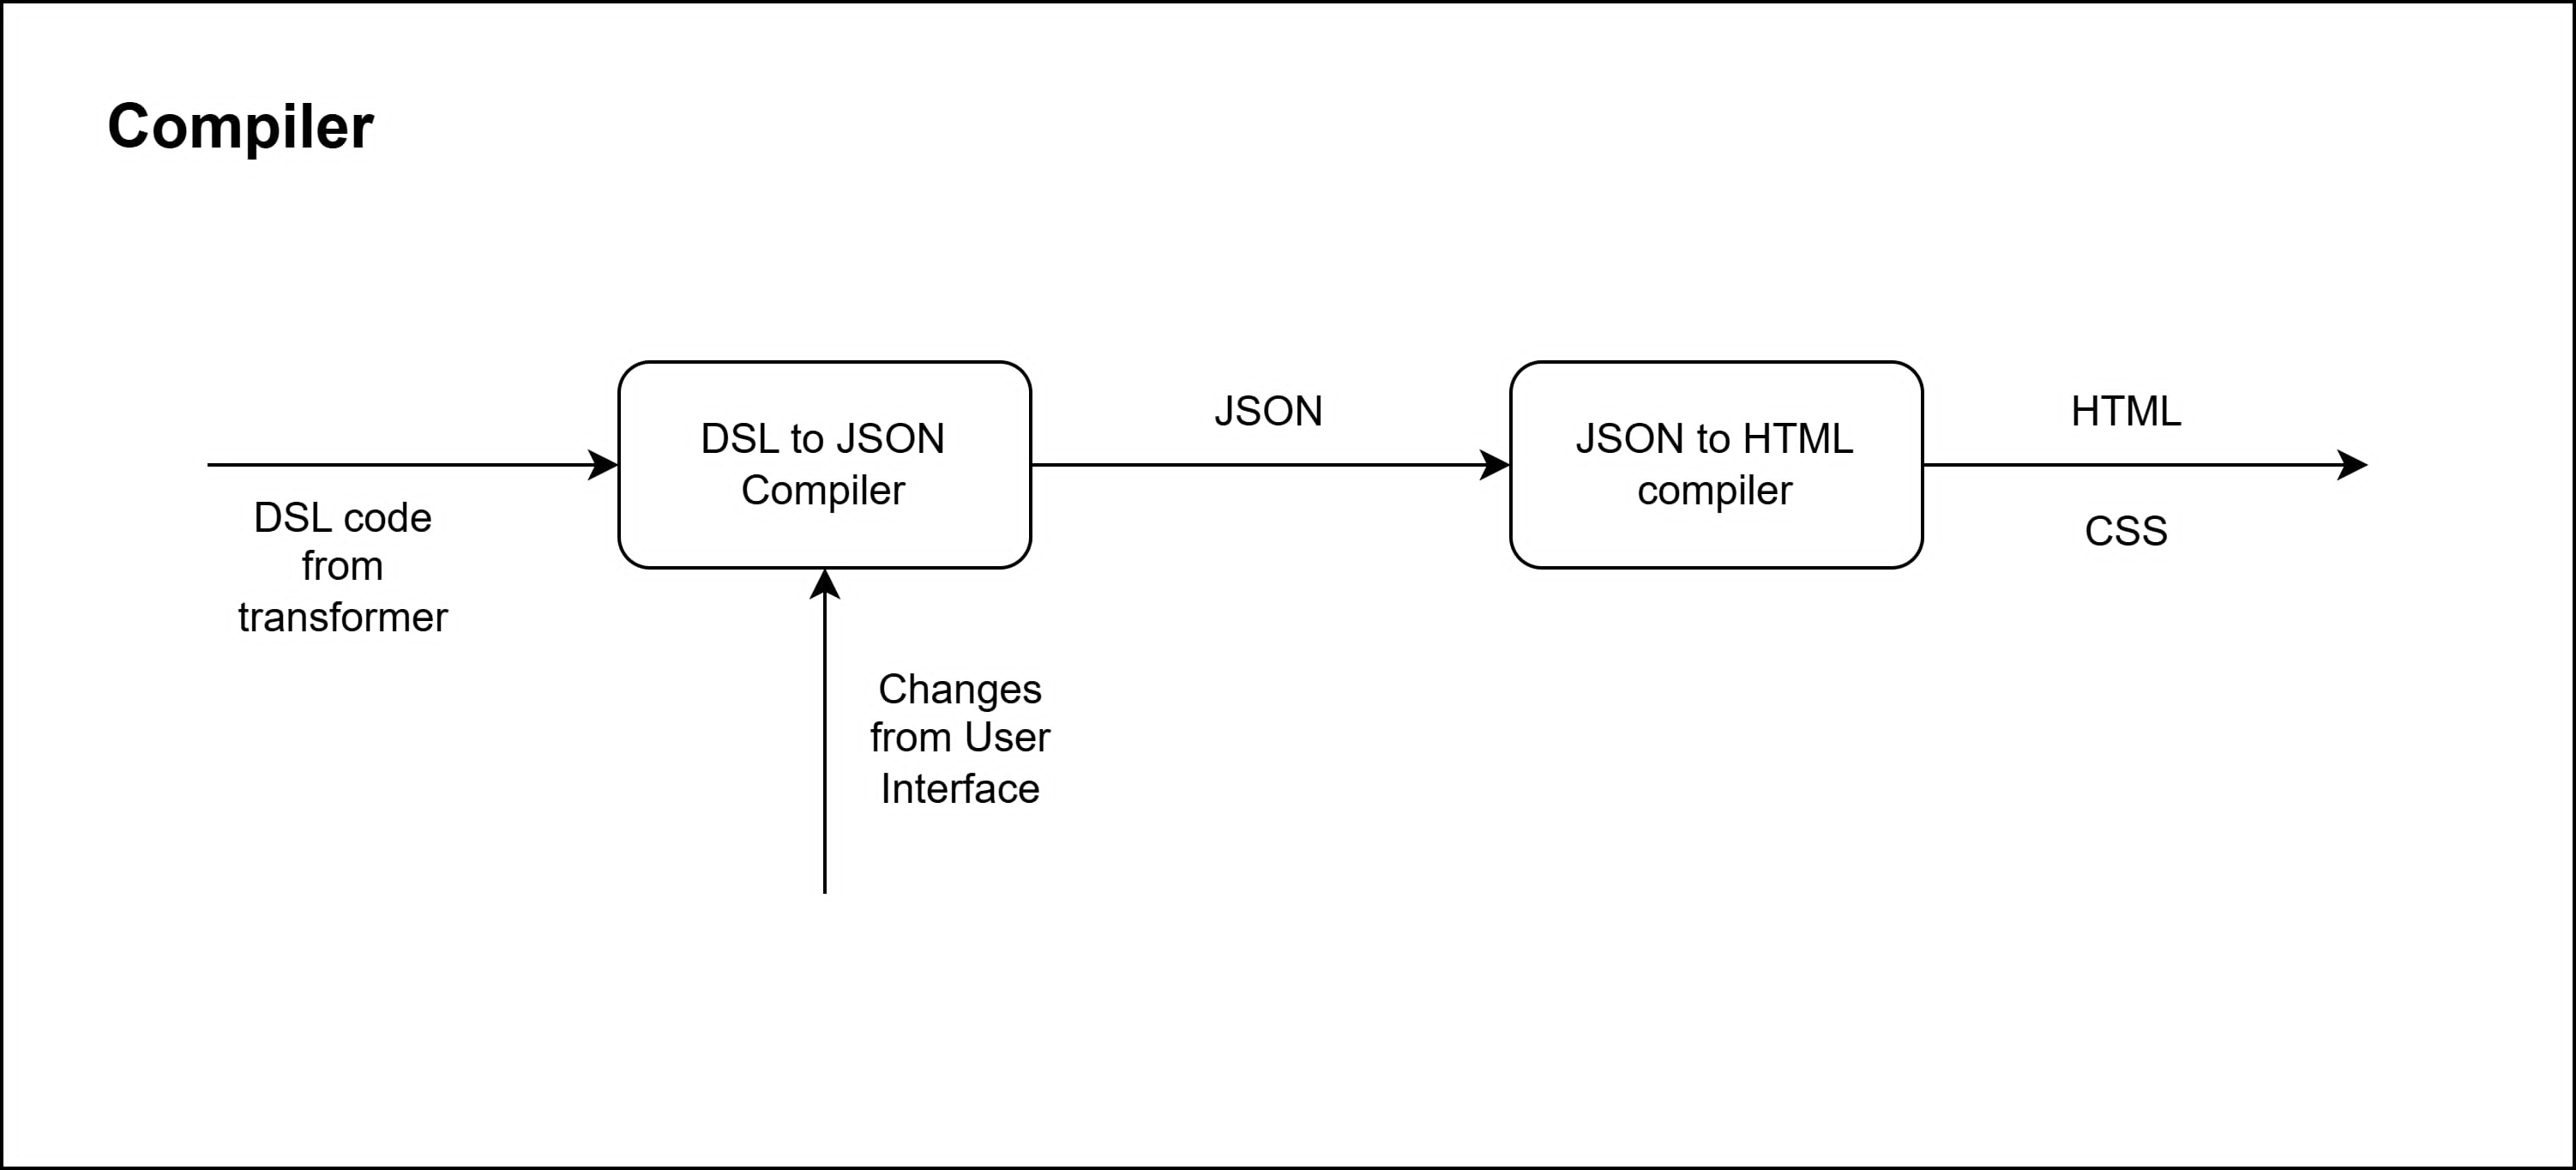
\includegraphics[scale=0.15, trim=100 200 200 0]{images/compiler flow.jpeg}
           \caption{Compiler Flow}
           \label{fig:Compflow}
       \end{figure}
   
 \subsection{Training Details}
 The model is trained using supervised learning with paired sketch-code data. It employs teacher forcing, where ground truth tokens are fed to the decoder during training to accelerate convergence and improve accuracy.

 \textbf{Objective Function}\\
 The training goal is to minimize cross-entropy loss between predicted and actual tokens, guiding the model to generate accurate DSL code sequences.

 \textbf{Optimization}\\
 Both convolutional and transformer layers are optimized simultaneously, ensuring effective feature extraction and mapping to DSL code.
The training process uses supervised learning, teacher forcing, and data augmentation to enhance accuracy and generalization in DSL code generation.
 \subsection{Testing Details}
 During testing, the model generates DSL code, predicting one token at a time. It processes the input sketch and sequentially predicts tokens, using previously generated tokens as input for subsequent predictions.

 \textbf{Evaluation Metrics}\\
 The model's performance is assessed using the following metrics:
 \begin{itemize}
    \item \textbf{BLEU (Bilingual Evaluation Understudy):} Measures the similarity between the generated code and the reference code by comparing n-grams.
    \item \textbf{ROUGE (Recall-Oriented Understudy for Gisting Evaluation):} Evaluates the recall aspect by measuring the overlap of word sequences between the generated and reference codes.
\end{itemize}
\textbf{Human Evaluation}\\
In addition to automated metrics, human evaluation is conducted to assess the quality and relevance of the generated DSL code. Experts review the code to ensure it aligns with the intended design and accurately represents the input sketch.
\pagebreak